% !TEX program = xelatex
\documentclass[12pt]{article}
\usepackage{iftex}
\ifPDFTeX
    \usepackage[T2A]{fontenc}
    \usepackage[utf8]{inputenc}
\else
    \usepackage{fontspec}
    \IfFontExistsTF{CMU Serif}
        {\setmainfont{CMU Serif}}
        {\IfFontExistsTF{Times New Roman}
            {\setmainfont{Times New Roman}}
            {\setmainfont{TeX Gyre Termes}}}
\fi
\usepackage[russian]{babel}
\usepackage{amsmath}
\usepackage{amssymb}
\usepackage{graphicx}
\usepackage{float}
\usepackage{array}
\usepackage{geometry}
\usepackage{hyperref}

\geometry{left=3cm, right=3cm, top=2cm, bottom=2cm}
\hypersetup{colorlinks=true, linkcolor=black, citecolor=black, urlcolor=black}
\sloppy

\begin{document}

\begin{titlepage}
    \centering
    {\large Московский физико-технический институт\\[0.3cm]
    Физтех-школа природоподобных, плазменных и ядерных технологий им. И.В. Курчатова\\[0.3cm]
    Кафедра моделирования ядерных процессов и технологий\par}

    \vspace{2.5cm}

    {\Large\bfseries Магистерская дипломная работа\par}

    \vspace{1.5cm}

    {\LARGE\bfseries Двухканальная модель памяти твэла: доплеровский и тепловой отклик импульса мощности\par}

    \vspace{2.5cm}

    \begin{flushright}
        \begin{tabular}{>{\raggedleft\arraybackslash}p{5cm}p{7cm}}
            Выполнил: & студент группы М07-405\\
            & Елесин Георгий Павлович\\[0.4cm]
            Направление: & 03.04.01 Прикладные математика и физика\\[0.4cm]
            Профиль: & Общая и прикладная физика\\[0.4cm]
            Специализация: & Суперкомпьютерное моделирование в прикладной физике\\[0.4cm]
            Научный руководитель: & Цибульский Виктор Филиппович\\
        \end{tabular}
    \end{flushright}

    \vfill

    {Москва, 2026}
\end{titlepage}

\tableofcontents
\newpage

\section{Введение}

Импульсное энерговыделение в ядерном топливе нельзя полностью описать статическим температурным коэффициентом реактивности. В стационарной записи доплеровская обратная связь часто сводится к выражению
\[
\rho_D=\alpha_D\Delta T_f.
\]
Такая форма полезна для малых квазистационарных отклонений, но в коротком переходном процессе температура топлива является не внешним параметром, а результатом предшествующей истории мощности. Поэтому в данной работе твэл рассматривается как динамический элемент памяти: импульс мощности записывает в топливе температурный след, а этот след затем имеет два выхода.

Первый выход является реактивностным. Нагрев топлива уширяет резонансы поглощения тяжёлых изотопов, увеличивает резонансный захват и создаёт отрицательную доплеровскую реактивность \cite{NRCFeedback2012,DOEGeneralTechnicalBase2013}. В предлагаемой постановке этот эффект записывается не как мгновенная функция средней температуры, а как свёртка истории мощности с реактивностным ядром:
\[
\rho_D(t)=
-\int_0^tK_D(t-s)P(s)\,ds.
\]
Второй выход является тепловым. Энергия, депонированная в топливе, не попадает в воду мгновенно: она проходит через топливо, зазор, оболочку и поверхность теплообмена. Поэтому вода видит не сам нейтронный пик, а запаздывающий тепловой поток:
\[
Q_{fw}(t)=
\int_0^tH_{fw}(t-s)P(s)\,ds.
\]
Итак, центральная модель работы имеет вид
\[
P(t)
\longrightarrow
\begin{cases}
I_D(t)=K_D*P, & \text{доплеровская реактивностная память},\\[3pt]
Q_{fw}(t)=H_{fw}*P, & \text{тепловой поток в воду}.
\end{cases}
\]

Цель работы состоит в построении этой двухканальной модели и проверке того, какие её элементы могут быть идентифицированы по расчётам GeN-Foam. Научная новизна состоит в замене статического коэффициента реактивности на геометрически определённое ядро памяти \(K_D(t)\), а также во введении второго ядра \(H_{fw}(t)\), описывающего задержанный тепловой выход к воде.

Важный результат работы является отрицательным в физическом, но положительным в методическом смысле. Рассмотренный GeN-Foam case не является режимом доплеровского самогашения: топливная обратная связь оказывается примерно на три порядка меньше внешней вставки реактивности. Поэтому расчёт используется как weak-coupled benchmark для проверки диагностики. По серии малых импульсов тепловой канал \(H_{fw}\) идентифицируется устойчиво, тогда как реактивностный канал \(K_D\) в данной постановке остаётся ниже уровня надёжного восстановления.

\begin{figure}[H]
\centering
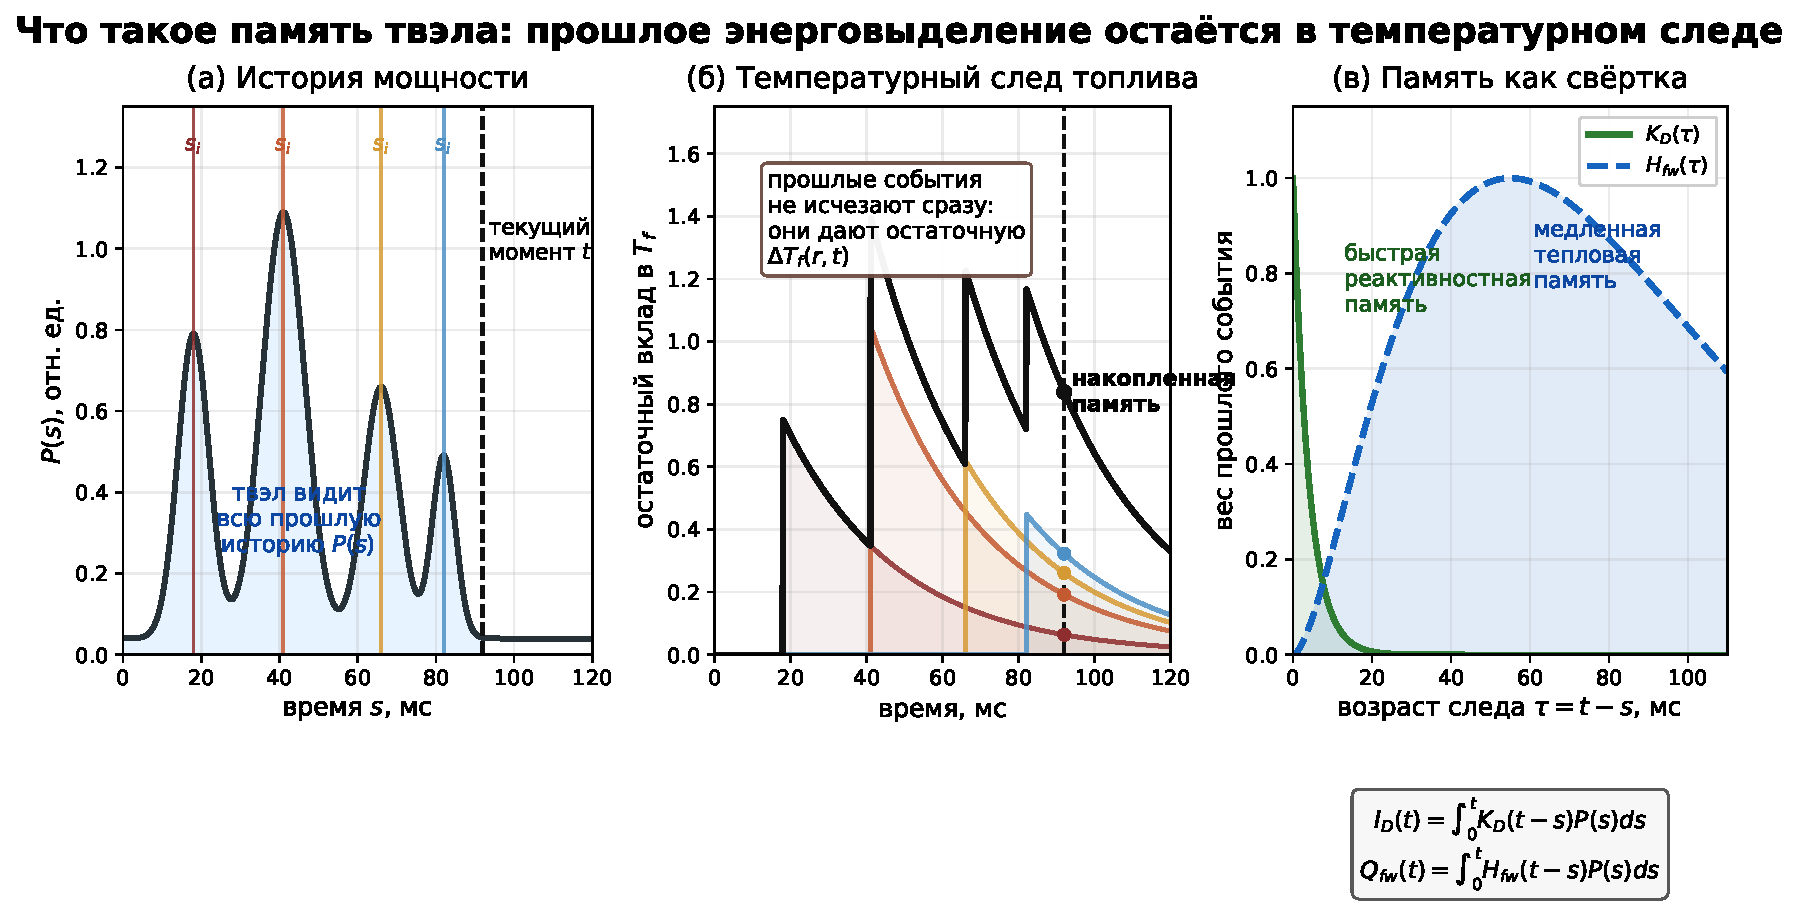
\includegraphics[width=\textwidth]{figures/fig0_fuel_memory_concept.pdf}
\caption{Физический смысл памяти твэла: история мощности создаёт остаточный температурный след, который затем взвешивается двумя ядрами памяти \(K_D\) и \(H_{fw}\).}
\label{fig:fuelMemoryConcept}
\end{figure}

\section{Двухканальная модель памяти твэла}

\subsection{Тепловой след и реактивностное ядро}

Рассмотрим топливную область \(\Omega_f\) и поверхность теплообмена с водой \(\Gamma_w\). На пониженном уровне описания пространственная форма энерговыделения отделяется от временной амплитуды:
\[
q'''(\mathbf r,t)=a(\mathbf r)P(t),
\qquad
\int_{\Omega_f}a(\mathbf r)\,dV=1.
\]
Температурный отклик топлива в линейном приближении записывается через функцию Грина теплопроводности:
\[
\Delta T_f(\mathbf r,t)=
\int_0^t\int_{\Omega_f}
G_T(\mathbf r,\mathbf r',t-s)
a(\mathbf r')P(s)\,dV'ds.
\]
Функция \(G_T\) содержит геометрию, теплопроводность, теплоёмкость и граничные условия. Именно она превращает историю мощности в распределённый температурный след.

Не всякий нагрев топлива одинаково важен для реактивности. Поэтому вводится поле доплеровской важности
\[
D_D(\mathbf r)=
-\frac{\delta\rho}{\delta T_f(\mathbf r)}>0.
\]
Тогда доплеровский вклад имеет вид
\[
\rho_D(t)=
-\int_{\Omega_f}D_D(\mathbf r)\Delta T_f(\mathbf r,t)\,dV
=
-\int_0^tK_D(t-s)P(s)\,ds,
\]
где
\[
K_D(\tau)=
\int_{\Omega_f}\int_{\Omega_f}
D_D(\mathbf r)
G_T(\mathbf r,\mathbf r',\tau)
a(\mathbf r')\,dV'dV.
\]
Эта формула является главным теоретическим объектом работы. В ней геометрия входит не как иллюстрация, а как часть оператора памяти: \(a(\mathbf r')\) задаёт место энерговыделения, \(G_T\) -- распространение тепла, а \(D_D(\mathbf r)\) -- реактивностную значимость нагрева.

\subsection{Тепловой канал к воде}

Тот же температурный след создаёт второй выход -- тепловой поток к воде:
\[
Q_{fw}(t)=
\int_{\Gamma_w}
\left[-\lambda_f\nabla T_f(\mathbf r,t)\cdot\mathbf n\right]dS.
\]
После подстановки решения через \(G_T\) получаем
\[
Q_{fw}(t)=
\int_0^tH_{fw}(t-s)P(s)\,ds,
\]
\[
H_{fw}(\tau)=
\int_{\Gamma_w}\int_{\Omega_f}
\left[
-\lambda_f\nabla_{\mathbf r}G_T(\mathbf r,\mathbf r',\tau)\cdot\mathbf n
\right]
a(\mathbf r')\,dV'dS.
\]
Следовательно, один импульс мощности не имеет единственного ``теплового времени''. Он быстро влияет на реактивность через объёмный нагрев топлива и позже проявляется на границе с водой.

\begin{figure}[H]
\centering
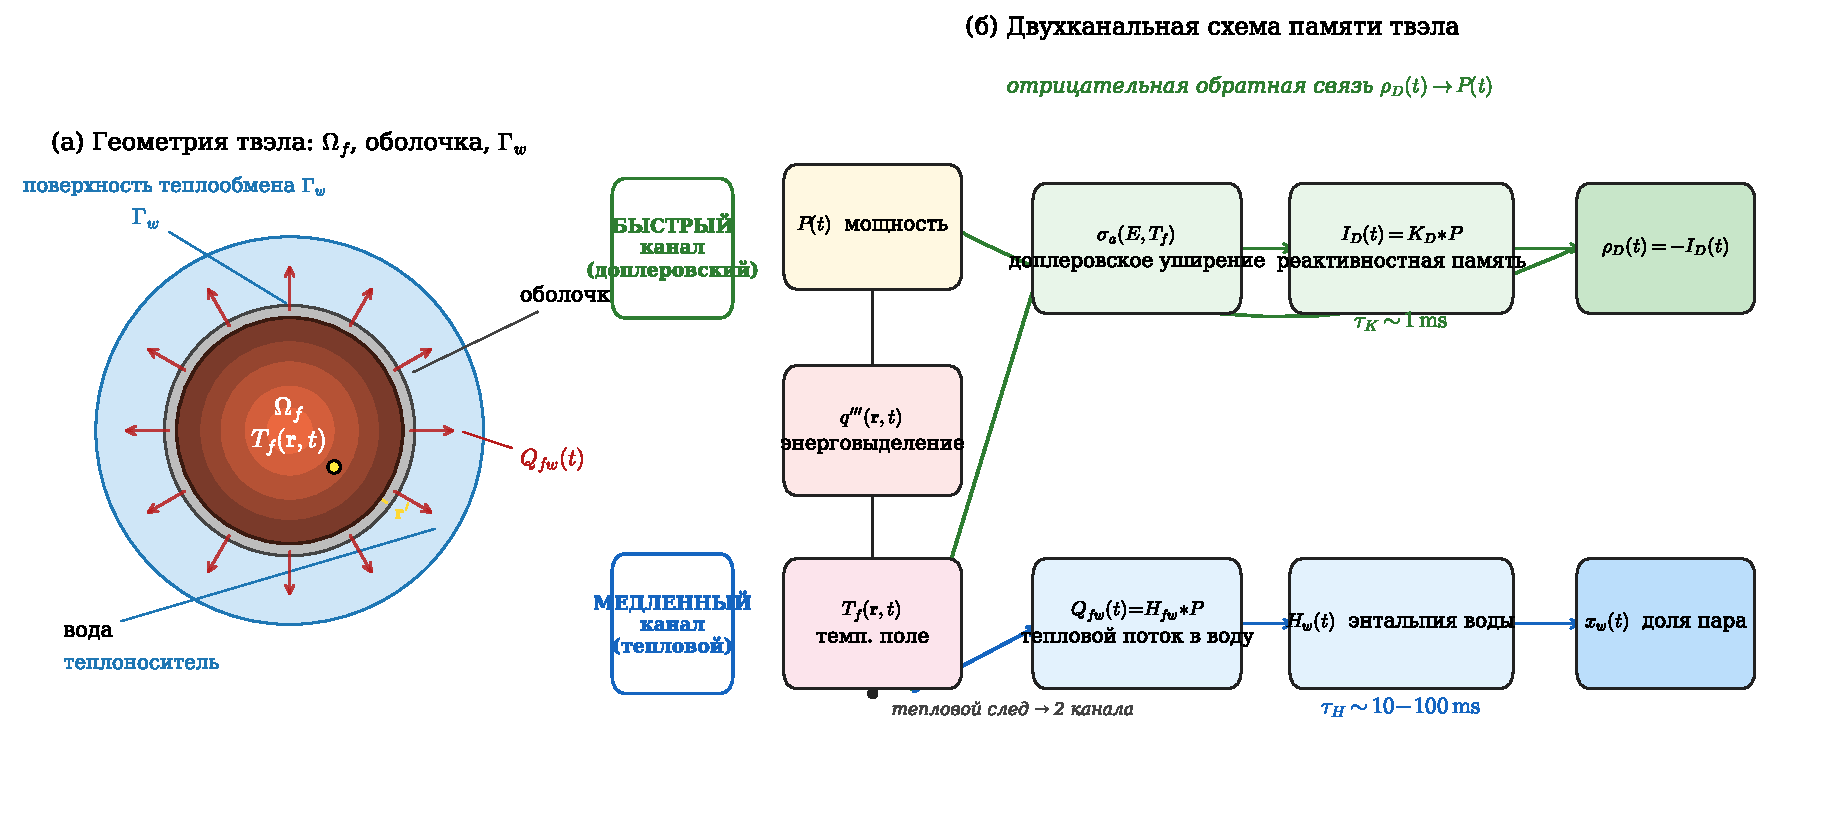
\includegraphics[width=\textwidth]{figures/fig1_twoChannel.pdf}
\caption{Двухканальная схема: история мощности \(P(t)\) создаёт быстрый реактивностный выход \(I_D=K_D*P\) и задержанный тепловой выход \(Q_{fw}=H_{fw}*P\).}
\label{fig:twoChannel}
\end{figure}

\subsection{Причинная структура свёрток}

Свёрточная форма модели подчёркивает, что текущий выход определяется не только текущей мощностью, но и всей предшествующей историей энерговыделения. Вклады мощности \(P(s)\,ds\), созданные в прошлые моменты времени, имеют разные физические веса: один набор весов задаёт реактивностный след топлива, другой -- тепловой выход к воде:
\[
I_D(t)=\int_0^tK_D(t-s)P(s)\,ds,
\qquad
Q_{fw}(t)=\int_0^tH_{fw}(t-s)P(s)\,ds.
\]
Соответственно,
\[
A_D(t,s)=K_D(t-s),
\qquad
A_W(t,s)=H_{fw}(t-s).
\]
Такое представление не является самостоятельной физической гипотезой; это компактная запись линейного причинного оператора, полученного из теплопроводности и реактивностной важности нагрева.

\subsection{Доплеровский механизм}

Физической причиной отрицательного реактивностного канала является температурное уширение резонансов. Температурно-уширенное сечение можно представить как усреднение неподвижного сечения по распределению скоростей ядер:
\[
\sigma_a^D(E,T_f)=
\int\sigma_a^{(0)}(E_{\mathrm{rel}})
M(\mathbf u_A;T_f)\,d^3u_A.
\]
При увеличении \(T_f\) резонансные пики сглаживаются по энергии, а эффективный резонансный захват возрастает. Для нейтронной кинетики это означает уменьшение вероятности избежать резонансного поглощения и появление отрицательного вклада в реактивность. В данной работе этот механизм используется как физическое основание для знака и смысла ядра \(K_D\); независимый расчёт температурно-зависимых сечений не выполнялся.

\begin{figure}[H]
\centering
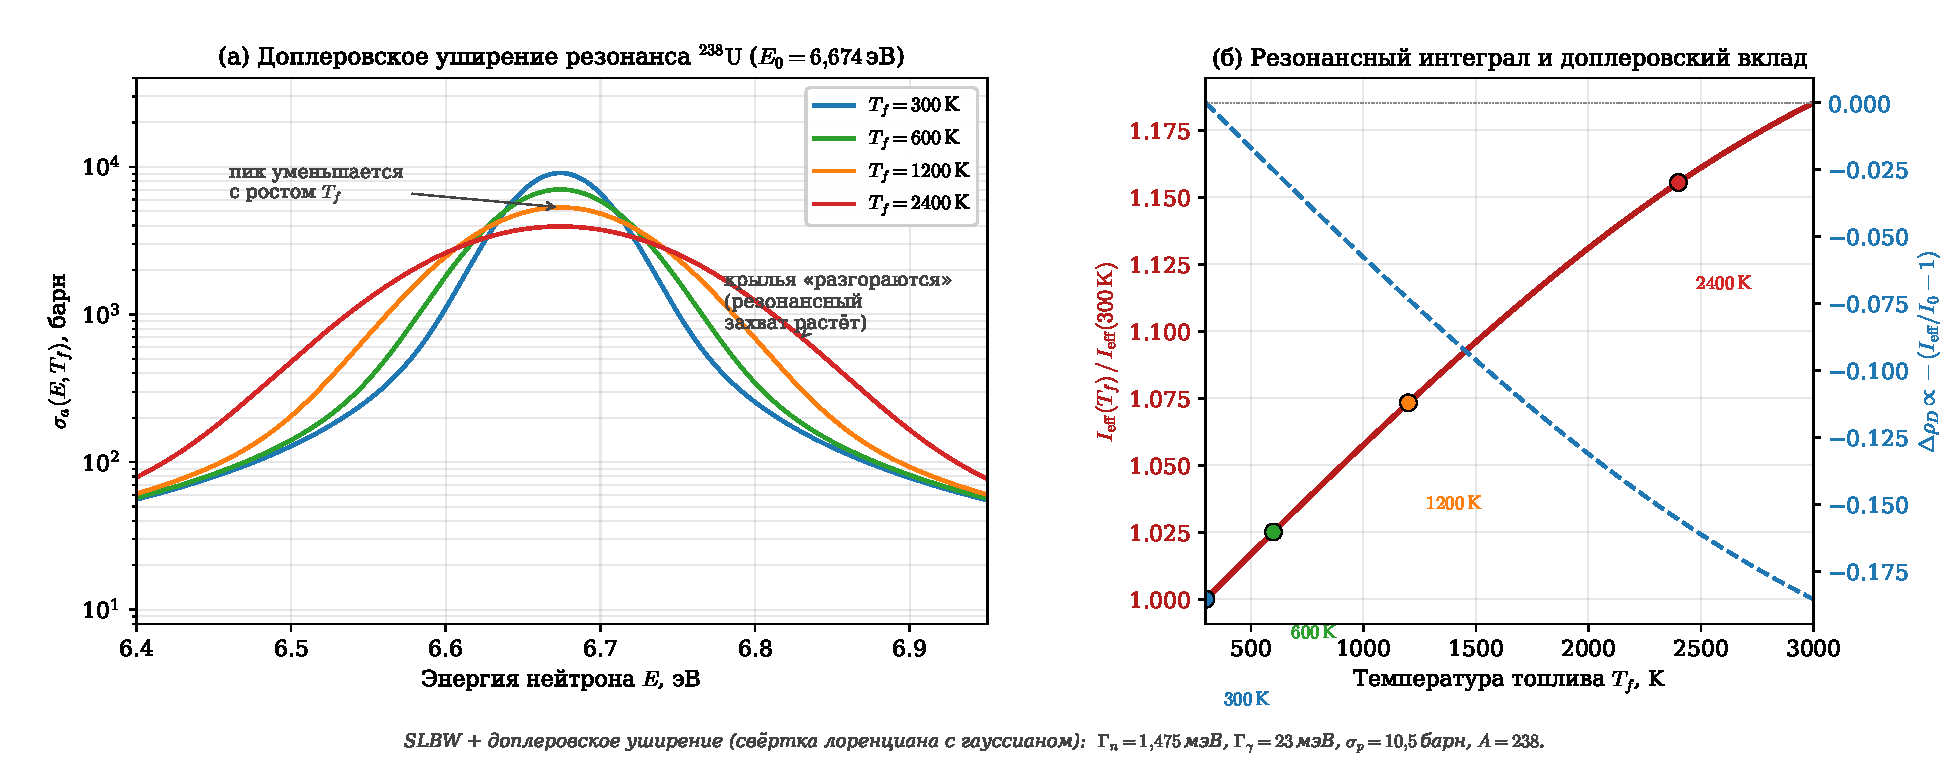
\includegraphics[width=\textwidth]{figures/fig2_doppler.pdf}
\caption{Иллюстративное доплеровское уширение резонанса \(^{238}\mathrm{U}\). Рисунок показывает качественный эффект уменьшения пика, расширения крыльев и роста эффективного резонансного интеграла; он не заменяет расчёт по библиотекам оценённых ядерных данных.}
\label{fig:doppler}
\end{figure}

\subsection{Кинетика и режимные критерии}

На уровне точечной кинетики с группами запаздывающих нейтронов \cite{DuderstadtHamilton1976}
\[
\frac{dP}{dt}=
\frac{\rho_{\mathrm{eff}}(t)-\beta}{\Lambda}P
+
\sum_i\lambda_iC_i+S(t),
\qquad
\frac{dC_i}{dt}=
\frac{\beta_i}{\Lambda}P-\lambda_iC_i.
\]
В модели памяти эффективная реактивность равна
\[
\rho_{\mathrm{eff}}(t)=
\rho_0-I_D(t)+\rho_{\mathrm{slow}}(t),
\qquad
I_D(t)=\int_0^tK_D(t-s)P(s)\,ds.
\]
Медленный функционал \(\rho_{\mathrm{slow}}\) может включать теплоноситель, плотность, паросодержание, давление и механику, но в данной работе он не является центральным объектом. Главный вопрос состоит в том, успевает ли \(I_D\) стать сравнимым с положительным реактивностным воздействием до того, как внешний импульс сам завершится.

Для классификации режимов вводятся два диагностических параметра. Первый сравнивает доплеровскую активацию с внешней вставкой:
\[
\mathcal D_{\mathrm{ext}}=
\frac{|I_D^{\max}|}{\rho_{\mathrm{ext}}^{\max}}.
\]
При необходимости сравнения с масштабом запаздывающих нейтронов используется
\[
\mathcal D_\beta=
\frac{I_D^{\max}}{\beta}.
\]
Условие \(\mathcal D_{\mathrm{ext}}\sim1\) является необходимым признаком доплеровски активного режима, но не является достаточным. Нужно также временное условие: характерное время роста ядра \(K_D\) должно быть не больше времени развития мощности,
\[
\tau_K \lesssim \tau_{\mathrm{growth}}.
\]
Если \(I_D\) становится заметным только после завершения внешнего импульса, такой расчёт остаётся внешне вынужденным даже при наличии отрицательной топливной обратной связи.

Второй параметр показывает долю энергии, дошедшую до водного канала за заданное время наблюдения:
\[
\mathcal W(t_{\mathrm{obs}})=
\frac{E_w(t_{\mathrm{obs}})}{E_{\mathrm{pulse}}},
\qquad
E_w(t)=\int_0^tQ_{fw}(s)\,ds.
\]
Запись \(\mathcal W\) без времени наблюдения неполна, потому что водный канал может иметь длинный хвост.

\begin{table}[H]
\centering
\caption{Основные величины модели и их размерности.}
\label{tab:units}
\begin{tabular}{|>{\centering\arraybackslash}p{3.1cm}|p{6.4cm}|>{\centering\arraybackslash}p{3.0cm}|}
\hline
Величина & Смысл & Единицы\\
\hline
\(P_{\mathrm{abs}}(t)\) & абсолютная мощность & W\\
\(\Delta P(t), u(t)\) & baseline-subtracted excess power & W\\
\(K_D(t)\) & реактивностное ядро & pcm/J или \(1/J\)\\
\(I_D(t)\) & доплеровская память & pcm\\
\(H_{fw}(t)\) & тепловое ядро & \(1/s\) или W/J\\
\(Q_{fw}(t)\) & поток в воду & W\\
\(E_w(t)\) & энергия в водный канал & J\\
\(\mathcal D_{\mathrm{ext}}, \mathcal W(t)\) & критерии режима & безразмерные\\
\hline
\end{tabular}
\end{table}

Функции памяти удобно аппроксимировать суммой экспонент:
\[
K_D(t)=\sum_jA_je^{-t/\tau_j},
\qquad
H_{fw}(t)=\sum_jB_je^{-t/\theta_j}.
\]
Тогда свёртки заменяются дополнительными переменными:
\[
\dot z_j=u-\frac{z_j}{\tau_j},
\quad
I_D=\sum_jA_jz_j,
\qquad
\dot y_j=u-\frac{y_j}{\theta_j},
\quad
Q_{fw}=\sum_jB_jy_j.
\]
Именно такая reduced-модель является рациональным расчётным уровнем для построения карты режимов; OpenFOAM и MOOSE в этой логике используются как источники или проверка параметров теплового слоя, а не как замена теории памяти \cite{MOOSEHeatTransfer,OpenFOAMSolvers}.

\begin{figure}[H]
\centering
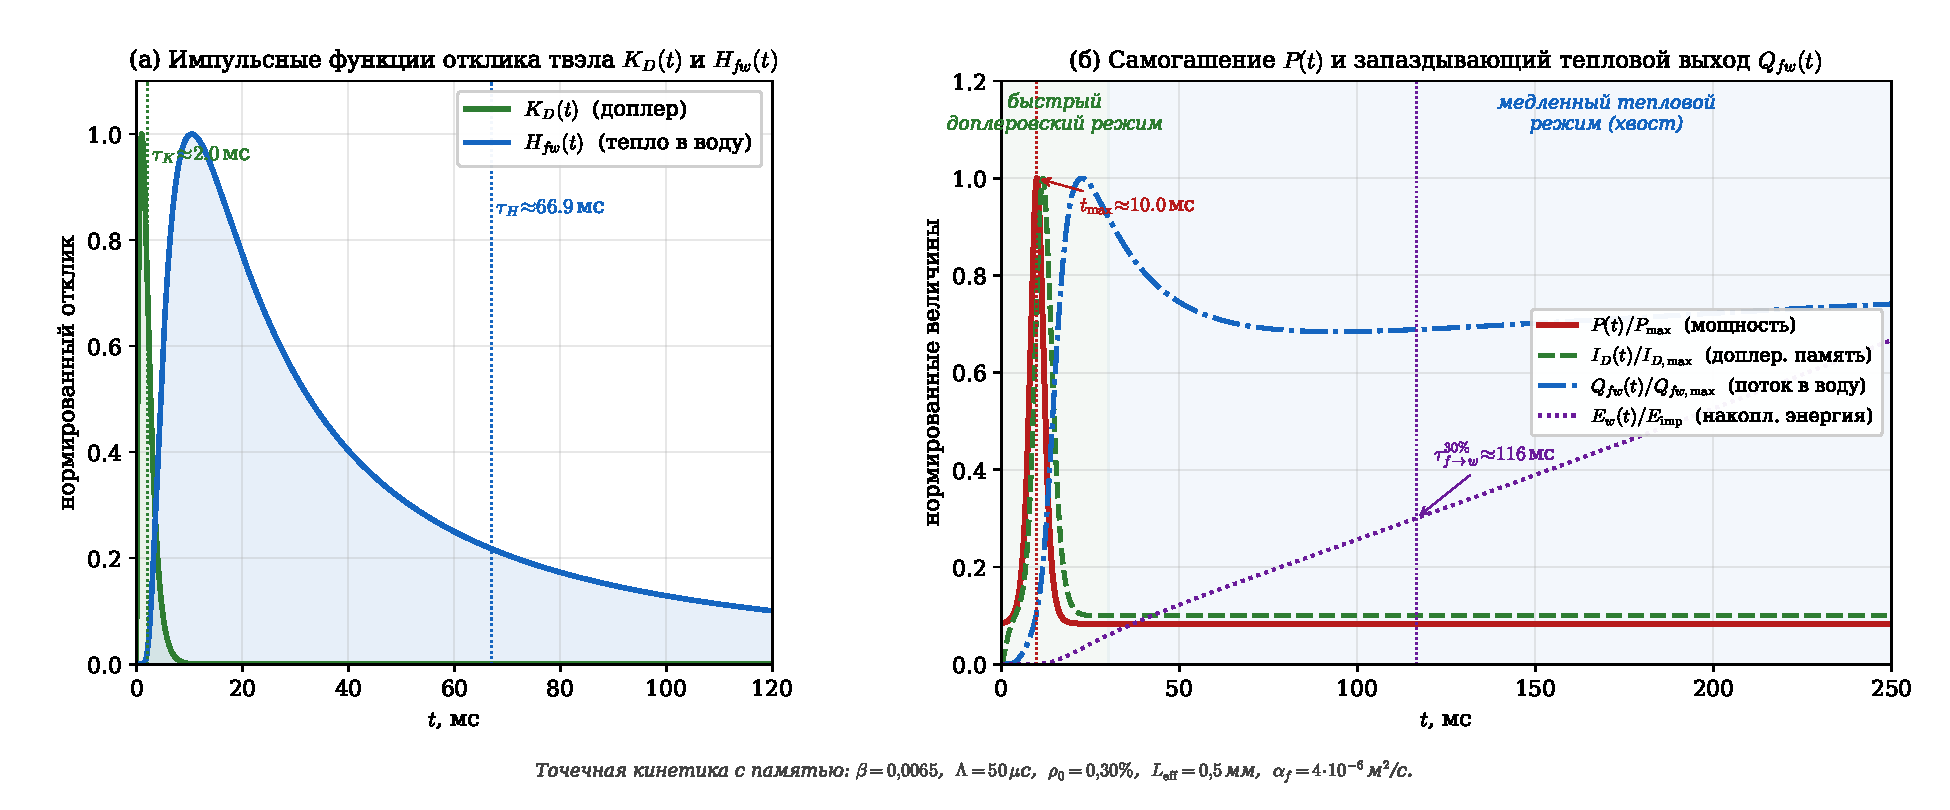
\includegraphics[width=\textwidth]{figures/fig3_dynamics.pdf}
\caption{Иллюстративный reduced-model расчёт, не соответствующий параметрам GeN-Foam benchmark. Он показывает целевой режим, в котором быстрый \(K_D\) ограничивает мощность раньше, чем \(H_{fw}\) передаёт существенную энергию в воду.}
\label{fig:dynamics}
\end{figure}

\subsection{Границы применимости}

Модель с двумя свёрточными ядрами корректна, пока допустимы разделение амплитуды и формы нейтронного поля
\[
f_n(\mathbf r,\mathbf p,t)\approx A(t)f_0(\mathbf r,\mathbf p)
\]
и квазистационарность формы энерговыделения
\[
a(\mathbf r,t)\approx a(\mathbf r).
\]
Если пространственная форма потока меняется во время импульса, если резонансная самозащита требует полного спектрального расчёта на каждом временном шаге, либо если двухфазная теплогидравлика становится сравнимой с быстрым доплеровским слоем, reduced-модель должна рассматриваться только как аппроксимация.

\section{Тепловые масштабы и связь с водой}

Тепловой канал нельзя оценивать по длительности нейтронного импульса. За время \(t\) тепловое возмущение в твёрдом топливе распространяется на глубину порядка
\[
\ell_T(t)\sim\sqrt{\alpha_f t},
\]
где \(\alpha_f=\lambda_f/(\rho_fc_{p,f})\). Для типичного порядка \(\alpha_f\sim10^{-6}\,\mathrm{m^2/s}\) за \(1\,\mathrm{ms}\) тепло проходит только десятки микрон. Поэтому локальный доплеровский нагрев может быть миллисекундным, а заметный выход энергии к воде -- существенно более поздним.

Грубая диффузионная оценка времени выхода тепла к поверхности имеет вид
\[
\tau_{f\to w}\sim
c_\eta\frac{L_{\mathrm{eff}}^2}{\alpha_f}
+
\frac{\delta_{\mathrm{barrier}}^2}{\alpha_b}.
\]
Здесь \(L_{\mathrm{eff}}\) -- эффективное расстояние от области энерговыделения до поверхности теплообмена, \(\delta_{\mathrm{barrier}}\) -- толщина промежуточного теплового барьера, а \(c_\eta\) зависит от выбранной доли энергии \(\eta\). Для идеализированного субмиллиметрового расстояния получаются оценки порядка \(10\)--\(100\,\mathrm{ms}\), но это не универсальная константа.

Именно поэтому результаты GeN-Foam нужно интерпретировать как эффективное ядро конкретной sub-scale постановки. В диагностической серии водный канал имеет секундный хвост: к \(3\,\mathrm{s}\) в воду уходит только около \(13.5\)--\(14.0\%\) excess-энергии, а время достижения \(10\%\) составляет примерно \(2.07\)--\(2.15\,\mathrm{s}\). Это не противоречит теории: аналитическая оценка описывает идеализированный путь теплопроводности, а GeN-Foam \texttt{nuclearFuelPin}/\texttt{heatFlux.structure} включает эффективную инерцию топлива, оболочки и sub-scale теплообмена.

\section{GeN-Foam и роль benchmark в работе}

GeN-Foam -- это открытый мультифизический расчётный код на базе OpenFOAM, предназначенный для моделирования переходных процессов в ядерных реакторах \cite{GeNFoam2015,foamForNuclear2026}. Его важная особенность состоит в том, что нейтроника, теплогидравлика и теплообмен в твёрдых структурах решаются в одной связанной постановке. В зависимости от выбранной модели GeN-Foam может использовать точечную кинетику или пространственную нейтронику, однофазную или двухфазную теплогидравлику, а также sub-scale модели твэлов и твёрдых конструкций.

В данной работе используется связка моделей \texttt{pointKinetics}, \texttt{onePhase} и \texttt{nuclearFuelPin}. Точечная кинетика задаёт динамику мощности и реактивности, однофазная теплогидравлика описывает теплоноситель, а модель \texttt{nuclearFuelPin} рассчитывает эффективный одномерный теплообмен внутри твэла и передаёт тепловой поток в жидкостную область. Поэтому GeN-Foam здесь не является инструментом прямого восстановления пространственного поля \(D_D(\mathbf r)\). Его роль более узкая: дать самосогласованные временные ряды мощности, температур, топливной обратной связи и теплового потока к воде в конкретной мультифизической постановке.

Под benchmark в этой работе понимается не экспериментальный эталон, а фиксированный воспроизводимый расчётный сценарий. Он задаёт начальное состояние, внешнюю вставку реактивности, набор физических моделей, сетку, параметры твэла, способ вывода полей и процедуру постобработки. Такой сценарий нужен для того, чтобы не обсуждать модель памяти только на уровне формул, а проверить, какие диагностические величины можно извлечь из реального coupled transient:
\[
P(t),\quad
\Delta\rho_f(t),\quad
T_f(t),\quad
Q_{fw}(t),\quad
E_w(t).
\]
Именно из этих временных рядов затем строятся baseline-subtracted сигналы, критерии \(\mathcal D_{\mathrm{ext}}\) и \(\mathcal W(t_{\mathrm{obs}})\), а также попытка идентификации ядер \(K_D\) и \(H_{fw}\).

Benchmark нужен в работе по трём причинам. Во-первых, он проверяет диагностическую процедуру: можно ли по расчётным данным отделить собственный отклик на импульс от фонового дрейфа. Во-вторых, он показывает, какой из двух каналов памяти реально виден в выбранной постановке. В-третьих, он служит контрпримером к целевому Doppler-active режиму: если \(\mathcal D_{\mathrm{ext}}\ll1\), то спад мощности нельзя честно объяснять доплеровским самогашением, даже если в модели присутствует отрицательная топливная обратная связь.

Таким образом, GeN-Foam benchmark в данной диссертации является проверкой применимости и идентифицируемости модели памяти, а не финальным доказательством сильного доплеровского режима. Теория формулирует, как должны выглядеть ядра \(K_D\) и \(H_{fw}\); benchmark показывает, что в выбранном расчёте тепловое ядро \(H_{fw}\) наблюдаемо, а реактивностное ядро \(K_D\) находится ниже уровня надёжного восстановления.

\section{GeN-Foam benchmark как weak-coupled case}

В качестве численной проверки использован GeN-Foam case pointKinetics + onePhase + nuclearFuelPin \cite{GeNFoam2015,foamForNuclear2026}. Этот расчёт не рассматривается как доказательство доплеровского самогашения. Его роль -- baseline-subtracted benchmark для проверки диагностики режима.

Для отделения реакции на импульс от фонового дрейфа рассчитывался контрольный вариант без внешней вставки реактивности. Далее все величины строились как
\[
\Delta X(t)=X_{\mathrm{pulse}}(t)-X_{\mathrm{baseline}}(t).
\]
Результат показан на рис.~\ref{fig:genfoamBaselineSubtracted}. Внешняя вставка реактивности создаёт заметный пик мощности, но топливная обратная связь остаётся на три порядка меньше внешнего воздействия.

\begin{figure}[H]
    \centering
    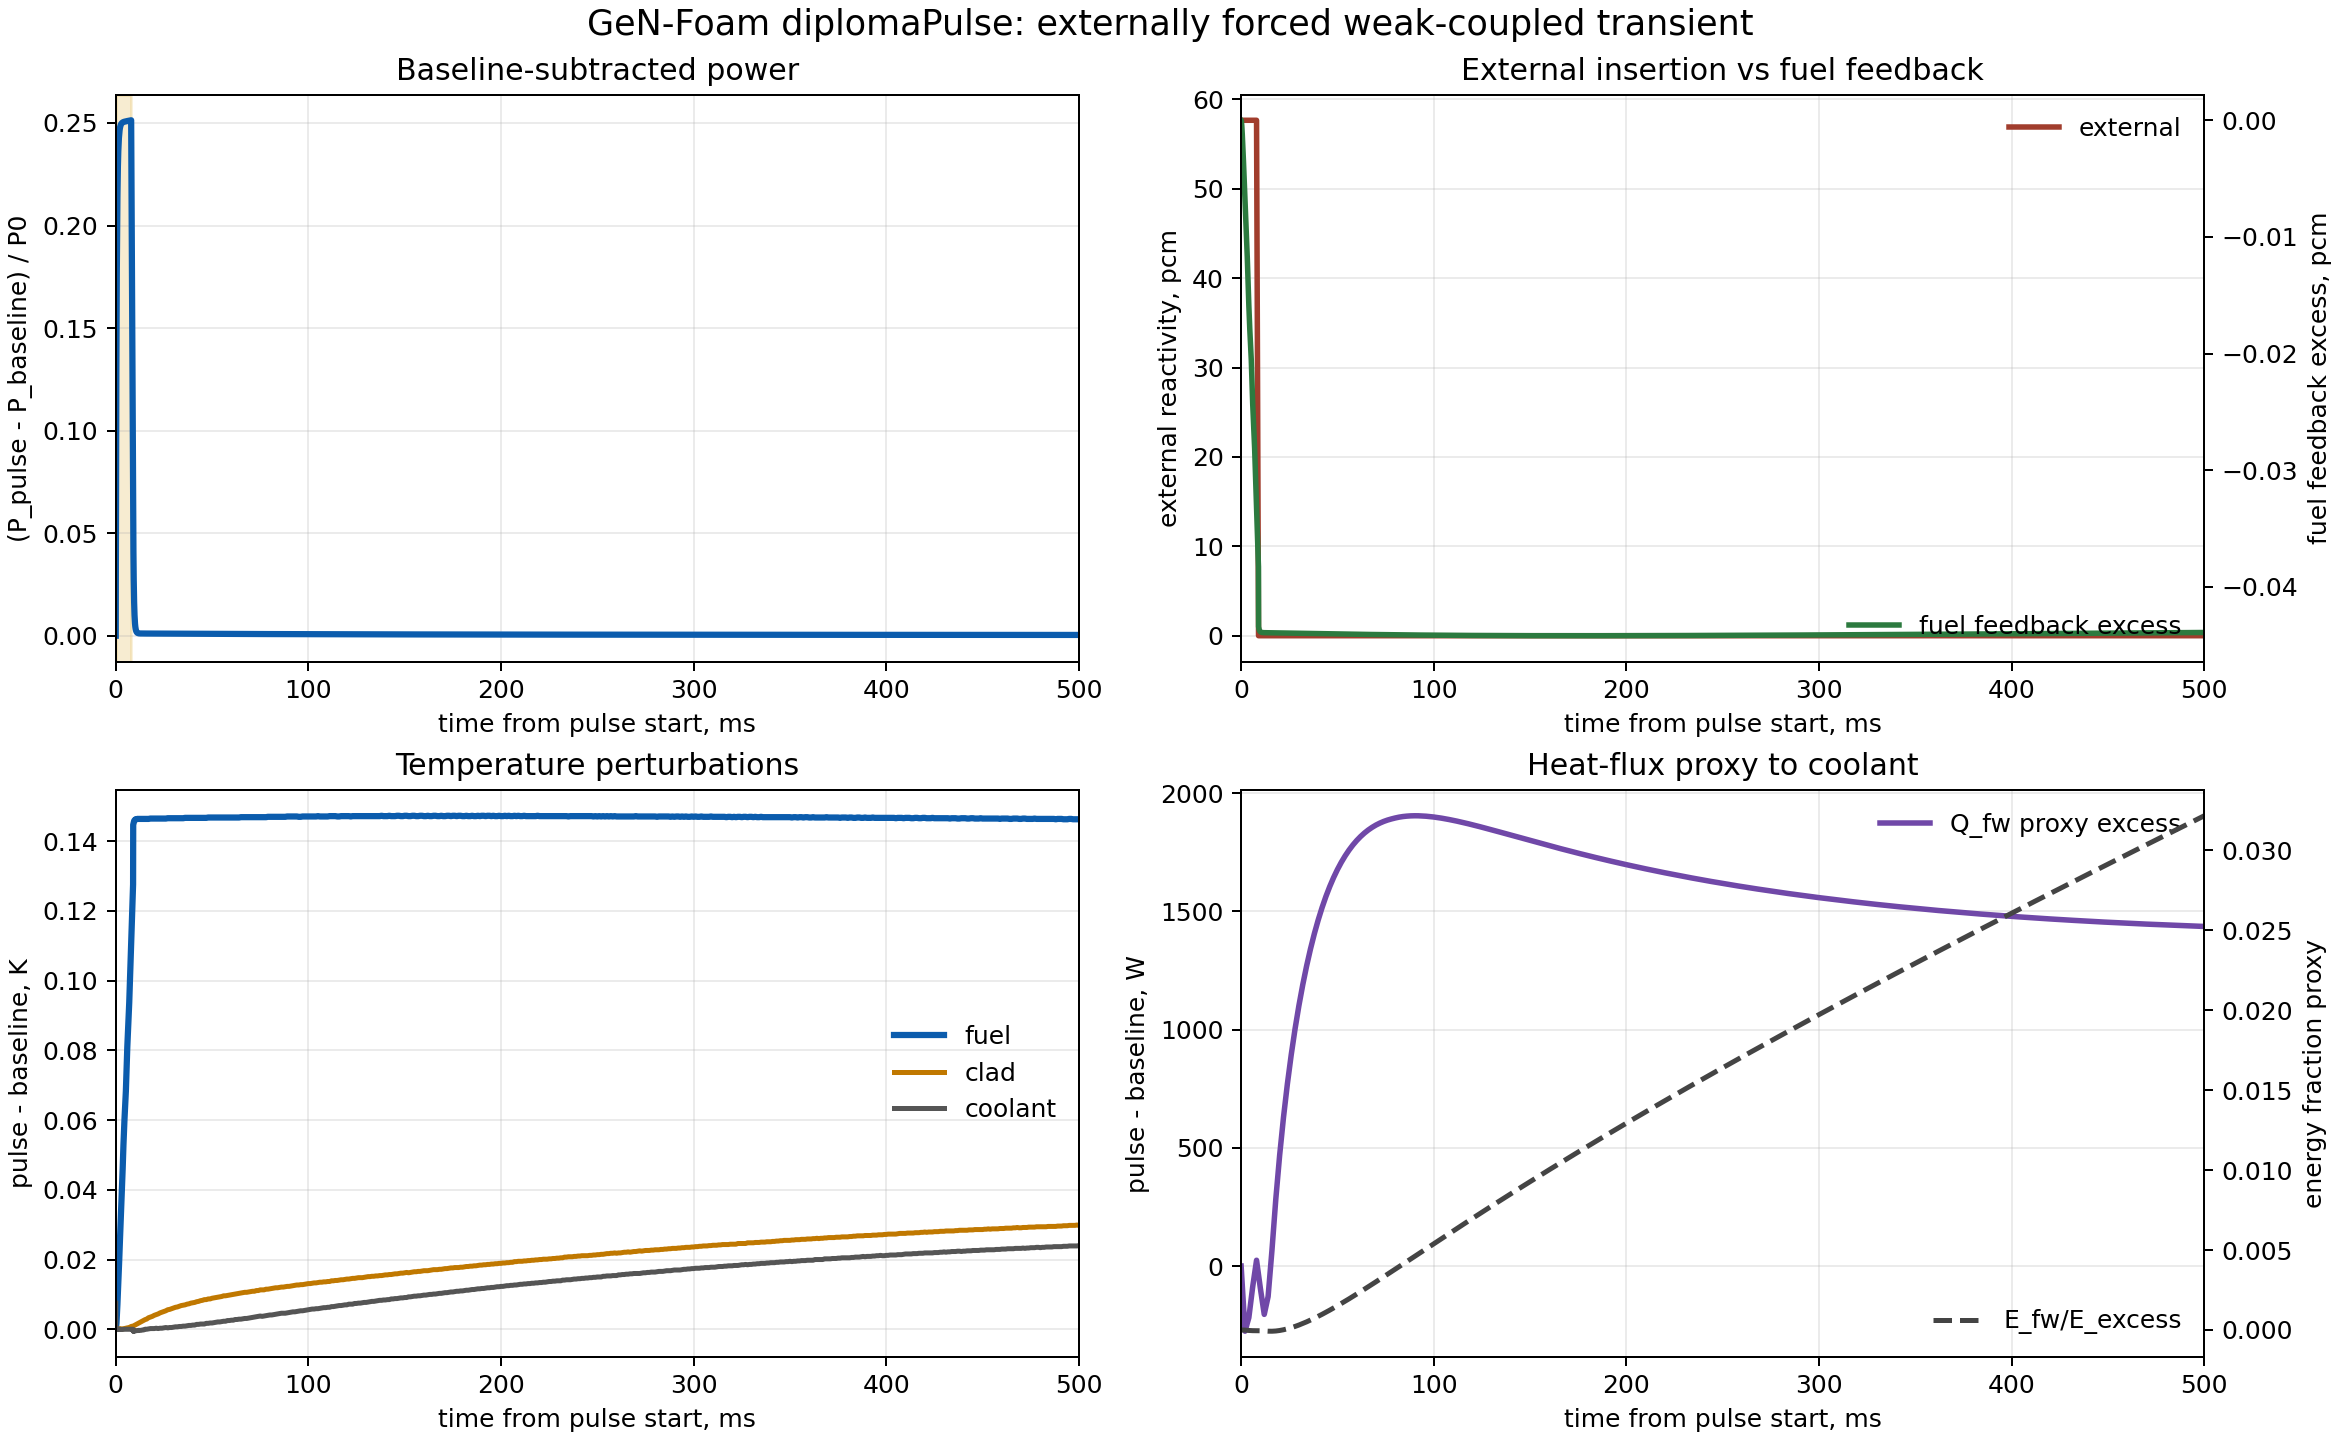
\includegraphics[width=\textwidth]{figures/fig4_genfoam_baseline_subtracted.png}
    \caption{Baseline-subtracted расчёт GeN-Foam. Спад мощности после \(8\,\mathrm{ms}\) связан главным образом с выключением внешней вставки, а не с доплеровским самогашением.}
    \label{fig:genfoamBaselineSubtracted}
\end{figure}

\begin{table}[H]
    \centering
    \caption{Численная диагностика проверочного GeN-Foam расчёта. Тепловой выход вычислен как подсеточный поверхностный интеграл $Q_{fw}=\sum_i q_i''a_{v,i}V_i$ по полю \texttt{heatFlux.structure} модели \texttt{nuclearFuelPin}.}
    \label{tab:genfoamRegimeMetrics}
    \begin{tabular}{>{\raggedright\arraybackslash}p{0.52\textwidth}>{\raggedright\arraybackslash}p{0.33\textwidth}}
        \hline
        Классификация режима & слабосвязанный внешне вынужденный переходный процесс\\
        $\rho_{\mathrm{ext}}^{\max}$ & 57.67 pcm\\
        $P_{\max}/P_0$ & 1.251 при $t=8.0$ ms\\
        $\max|\Delta\rho_{f}|$ & 0.0442 pcm\\
        $\mathcal D=\max|\Delta\rho_f|/\rho_{\mathrm{ext}}^{\max}$ & $7.66\cdot 10^{-4}$\\
        $\max\Delta T_f$ & 0.147 K\\
        $\alpha_{\mathrm{eff}}$ & -0.300 pcm/K\\
        $E_{\text{имп}}$ & 23.87 kJ\\
        $\mathcal W(500\ \mathrm{ms})$ & 0.032\\
        $t_{10\%}$ по $E_w/E_{\text{имп}}$ & ---\\
        \hline
    \end{tabular}
\end{table}


Ключевые числа:
\[
\rho_{\mathrm{ext}}^{\max}=57.67\ \mathrm{pcm},
\qquad
\max|\Delta\rho_f|=0.0442\ \mathrm{pcm},
\]
\[
\mathcal D_{\mathrm{ext}}=
\frac{0.0442}{57.67}
=7.66\cdot10^{-4}.
\]
Следовательно, данный case является externally forced weak-coupled transient. Он не подтверждает центральную доплеровскую модель как режим самогашения; он показывает, что диагностика способна распознать отсутствие сильной доплеровской активации.

В текущей постановке \texttt{nuclearFuelPin} поверхность теплообмена не является явным patch сетки. Поэтому интегральный поток к воде вычисляется как sub-scale поверхностный интеграл
\[
Q_{fw}(t)=\sum_i q_i''(t)a_{v,i}V_i,
\]
где \(q_i''\) берётся из поля \texttt{heatFlux.structure}, а \(a_v=2\alpha_{\mathrm{structure}}/r_{\mathrm{clad}}\). Эта величина пригодна для диагностики теплового канала \(H_{fw}\), но не должна смешиваться с доказательством доплеровского самогашения.

Важно также разделять теоретическую 3D-формулу для \(K_D\) и фактический уровень разрешения GeN-Foam case. Поле доплеровской важности \(D_D(\mathbf r)\) в данном расчёте не восстанавливается как пространственное поле; GeN-Foam используется для интегральной диагностики отклика. Полноценная проверка геометрического функционала \(K_D\) требует либо разрешённого топливного benchmark, либо независимых статических perturbation-расчётов нейтроники при разных температурах топлива.

\section{Идентификация \(H_{fw}\) по диагностической серии}

Для восстановления функций памяти выполнена серия малых импульсов с одинаковой амплитудой внешней реактивности и разными длительностями:
\[
\tau_p=2,\ 4,\ 8,\ 16,\ 32\,\mathrm{ms},
\qquad
t_{\mathrm{end}}=3\,\mathrm{s}.
\]
Входом идентификационной задачи является
\[
u(t)=P_{\mathrm{pulse}}(t)-P_{\mathrm{baseline}}(t),
\]
а выходами являются
\[
y_D(t)=-
\left[
\rho_{f,\mathrm{pulse}}(t)-\rho_{f,\mathrm{baseline}}(t)
\right],
\qquad
y_w(t)=
Q_{fw,\mathrm{pulse}}(t)-Q_{fw,\mathrm{baseline}}(t).
\]
Искомые ядра должны удовлетворять
\[
y_D(t)\approx \int_0^tK_D(t-s)u(s)\,ds,
\qquad
y_w(t)\approx \int_0^tH_{fw}(t-s)u(s)\,ds.
\]
Здесь \(u(t)\) не является независимым управляющим сигналом внешнего эксперимента: мощность сама формируется реактивностью и обратными связями. Для теплового канала это допустимо как post-processing, потому что наблюдаемая excess-мощность является фактическим источником тепла. Для реактивностного канала ситуация хуже: \(y_D\) входит обратно в кинетику мощности, а сам сигнал мал по сравнению с внешней вставкой. Поэтому восстановление \(K_D\) в текущем closed-loop case трактуется только как проверка идентифицируемости, а не как измерение физического ядра.

\begin{table}[H]
    \centering
    \caption{Диагностическая серия GeN-Foam. Первая строка соответствует исходному 500 ms benchmark, остальные строки -- расчётам до \(3\,\mathrm{s}\); поэтому \(\eta_w(0.5s)\) и \(\eta_w(t_f)\) нужно сравнивать отдельно.}
    \label{tab:diagnosticSeries}
    \resizebox{\textwidth}{!}{\begin{tabular}{rrrrrrrrrr}
\hline
$\tau_p$, ms & $E_{\text{имп}}$, kJ & $P_{\max}/P_0$ & $\max|\rho_f|$, pcm & $\mathcal D$ & $E_w(0.5s)$, J & $E_w(t_f)$, J & $\eta_w(0.5s)$ & $\eta_w(t_f)$ & $t_{10\%}$, s\\
\hline
8 & 23.9 & 1.251 & 0.04418 & 0.000766 & 768 & 768 & 0.0322 & 0.0322 & ---\\ 
2 & 7.2 & 1.246 & 0.01023 & 0.000177 & 171 & 977 & 0.0238 & 0.136 & 2.15\\ 
4 & 14.8 & 1.250 & 0.02148 & 0.000372 & 363 & 2.04e+03 & 0.0245 & 0.138 & 2.11\\ 
8 & 30.1 & 1.251 & 0.04418 & 0.000766 & 768 & 4.2e+03 & 0.0255 & 0.14 & 2.07\\ 
16 & 60 & 1.253 & 0.08545 & 0.00148 & 1.5e+03 & 8.22e+03 & 0.025 & 0.137 & 2.12\\ 
32 & 120 & 1.255 & 0.1682 & 0.00292 & 2.91e+03 & 1.62e+04 & 0.0243 & 0.135 & 2.15\\ 
\hline
\end{tabular}
}
\end{table}

Главный результат серии состоит в различии идентифицируемости двух каналов. Тепловой выход \(\Delta Q_{fw}/E_{\mathrm{pulse}}\) и накопленная доля \(E_w/E_{\mathrm{pulse}}\) имеют близкую форму для разных длительностей импульса. Это означает, что в рассматриваемой области тепловой канал хорошо описывается линейным причинным ядром \(H_{fw}\). Реактивностный сигнал \(y_D\) значительно слабее: даже для \(\tau_p=32\,\mathrm{ms}\) \(\mathcal D_{\mathrm{ext}}\) остаётся порядка \(10^{-3}\), поэтому \(K_D\) в данной постановке не восстанавливается надёжно.

\begin{figure}[H]
    \centering
    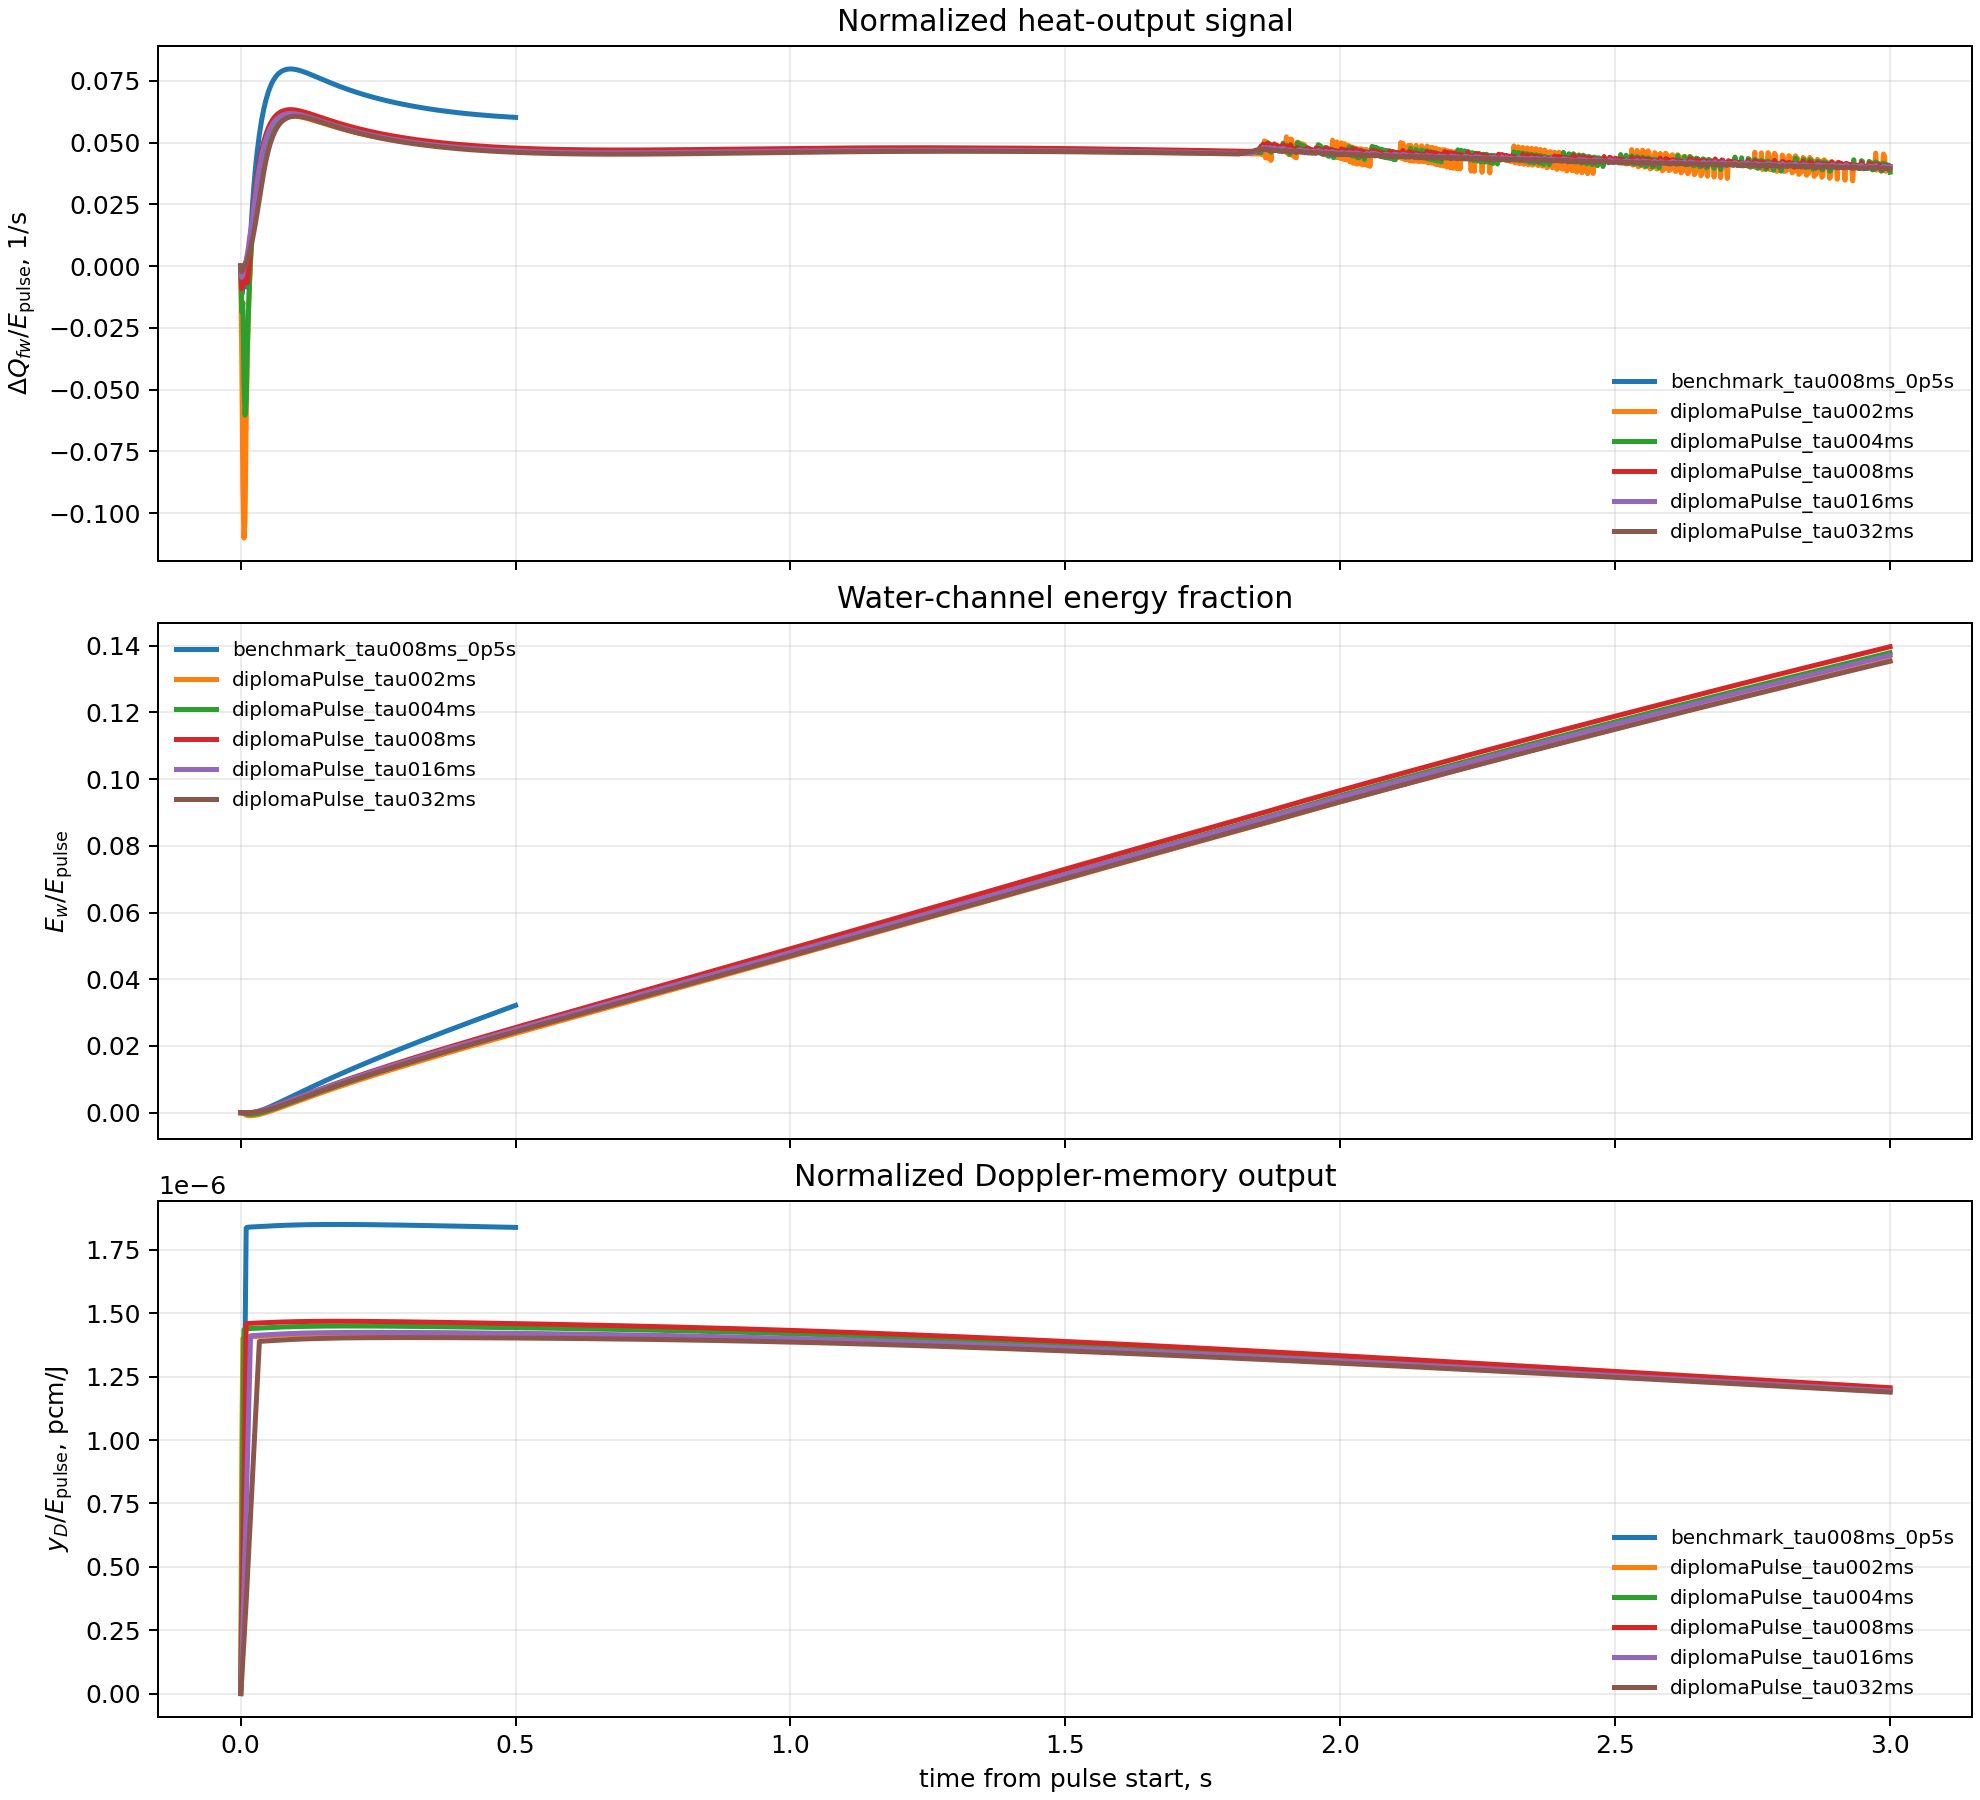
\includegraphics[width=\textwidth]{figures/fig8_diagnostic_normalized_overlays.png}
    \caption{Нормированные отклики диагностической серии. Тепловой канал коллапсирует лучше реактивностного, что указывает на устойчивую идентификацию \(H_{fw}\) и слабую идентифицируемость \(K_D\).}
    \label{fig:diagnosticOverlays}
\end{figure}

На раннем фронте \(Q_{fw}\) возможны малые отрицательные значения после baseline-subtraction. Они не интерпретируются как физический тепловой поток из воды в топливо: для положительного импульса мощности ожидаемое физическое ядро \(H_{fw}\) должно быть неотрицательным. Этот участок отражает чувствительность к вычитанию baseline, sign convention поля \texttt{heatFlux.structure} и начальному согласованию расчёта; поэтому выводы по \(H_{fw}\) опираются прежде всего на нормированную форму после фронта, накопленную энергию и leave-one-out проверку.

На карте режимов диагностическая серия остаётся в области weak forced transient по доплеровскому критерию, но при \(t_{\mathrm{obs}}=3\,\mathrm{s}\) пересекает уровень \(\mathcal W=0.1\). Следовательно, водный канал не отсутствует; он просто имеет длинную память и проявляется позже нейтронного пика.

Рис.~\ref{fig:diagnosticRegimeMap} следует читать с учётом времени наблюдения: исходный benchmark показан при \(t_{\mathrm{obs}}=0.5\,\mathrm{s}\), а диагностические runs -- при \(t_{\mathrm{obs}}=3\,\mathrm{s}\). Поэтому карта иллюстрирует режимную классификацию, но честное сравнение теплового выхода между cases проводится по двум отдельным столбцам таблицы~\ref{tab:diagnosticSeries}: \(\eta_w(0.5s)\) и \(\eta_w(t_f)\).

\begin{figure}[H]
    \centering
    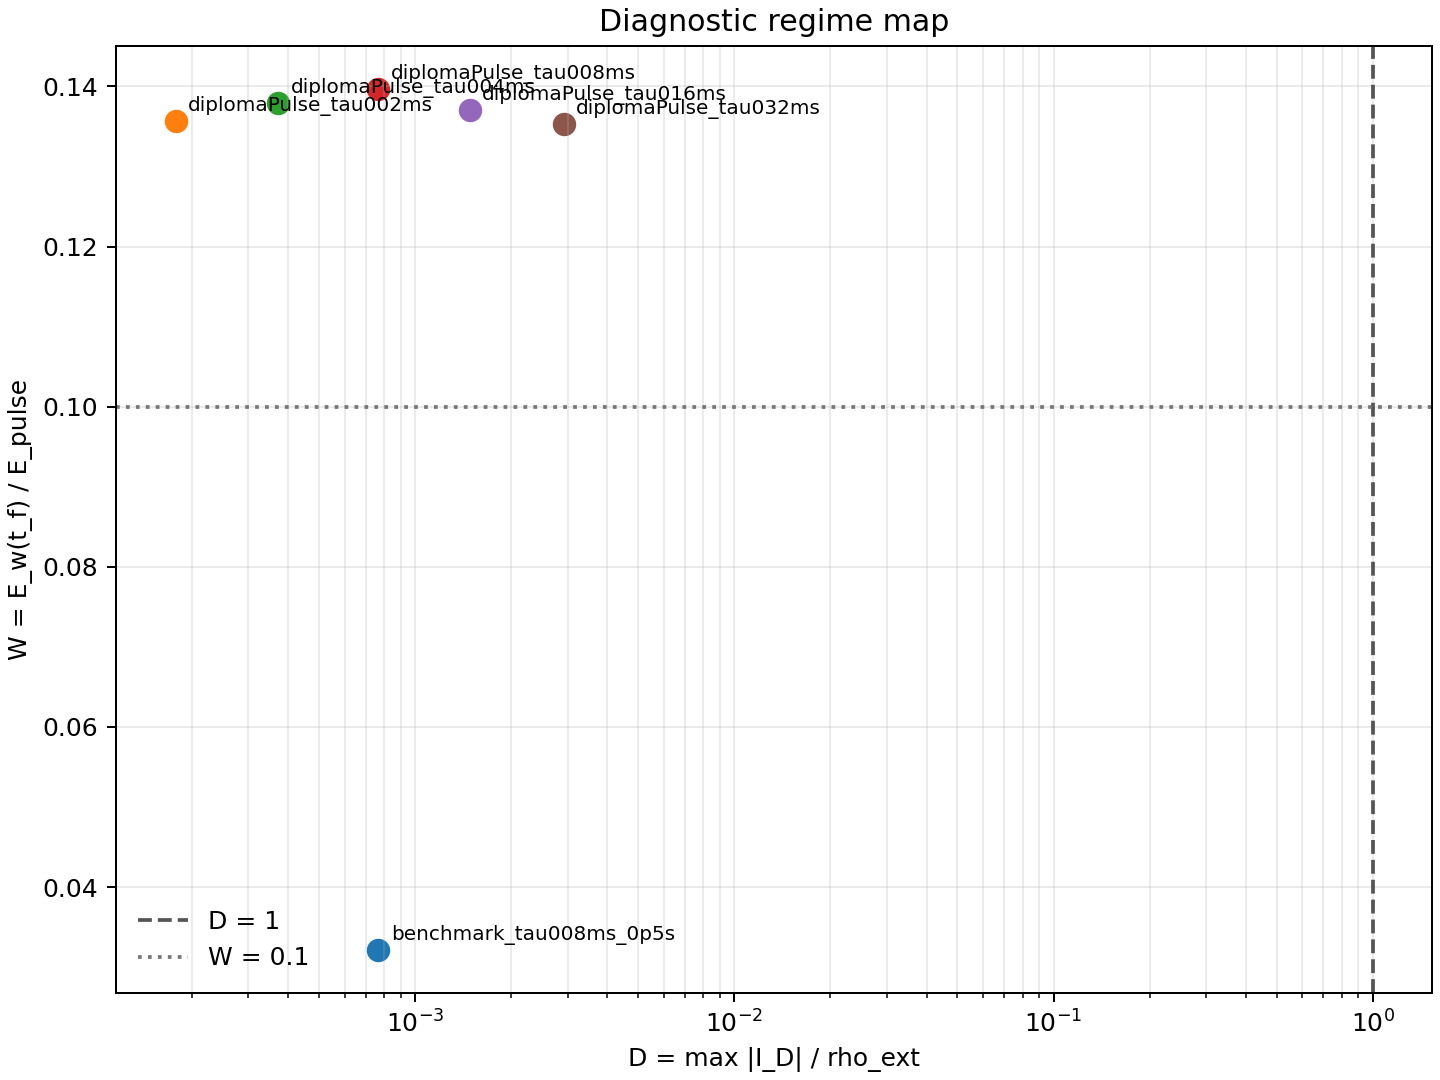
\includegraphics[width=0.82\textwidth]{figures/fig9_diagnostic_regime_map.png}
    \caption{Карта режимов в координатах \(\mathcal D_{\mathrm{ext}}\) и \(\mathcal W(t_{\mathrm{obs}})\). Исходный benchmark имеет \(t_{\mathrm{obs}}=0.5\,\mathrm{s}\), диагностические cases -- \(t_{\mathrm{obs}}=3\,\mathrm{s}\); все точки остаются при \(\mathcal D_{\mathrm{ext}}\ll1\).}
    \label{fig:diagnosticRegimeMap}
\end{figure}

При физической идентификации ядра должны удовлетворять знаковым и энергетическим ограничениям:
\[
H_{fw}(t)\ge0,
\qquad
\int_0^\infty H_{fw}(t)\,dt\le1,
\qquad
K_D(t)\ge0
\]
при записи \(y_D=-\Delta\rho_f\). Поэтому sign-changing fit \(K_D\) не рассматривается как физическое ядро. Он показывает только, что weak-coupled GeN-Foam case не содержит достаточно сильного реактивностного сигнала для устойчивого восстановления \(K_D\).

Совместный fit теплового канала с неотрицательными коэффициентами \(B_j\) и временами
\[
\theta_j=0.05,\ 0.2,\ 1,\ 3,\ 10\,\mathrm{s}
\]
даёт \(R^2\approx0.987\) для \(H_{fw}\). Среднее время памяти fitted kernel составляет около \(8.8\,\mathrm{s}\), что превышает расчётное окно и потому должно пониматься как признак длинного хвоста, а не как окончательно измеренная асимптотическая константа. Для \(K_D\) аналогичная процедура даёт низкое качество восстановления.

\begin{figure}[H]
    \centering
    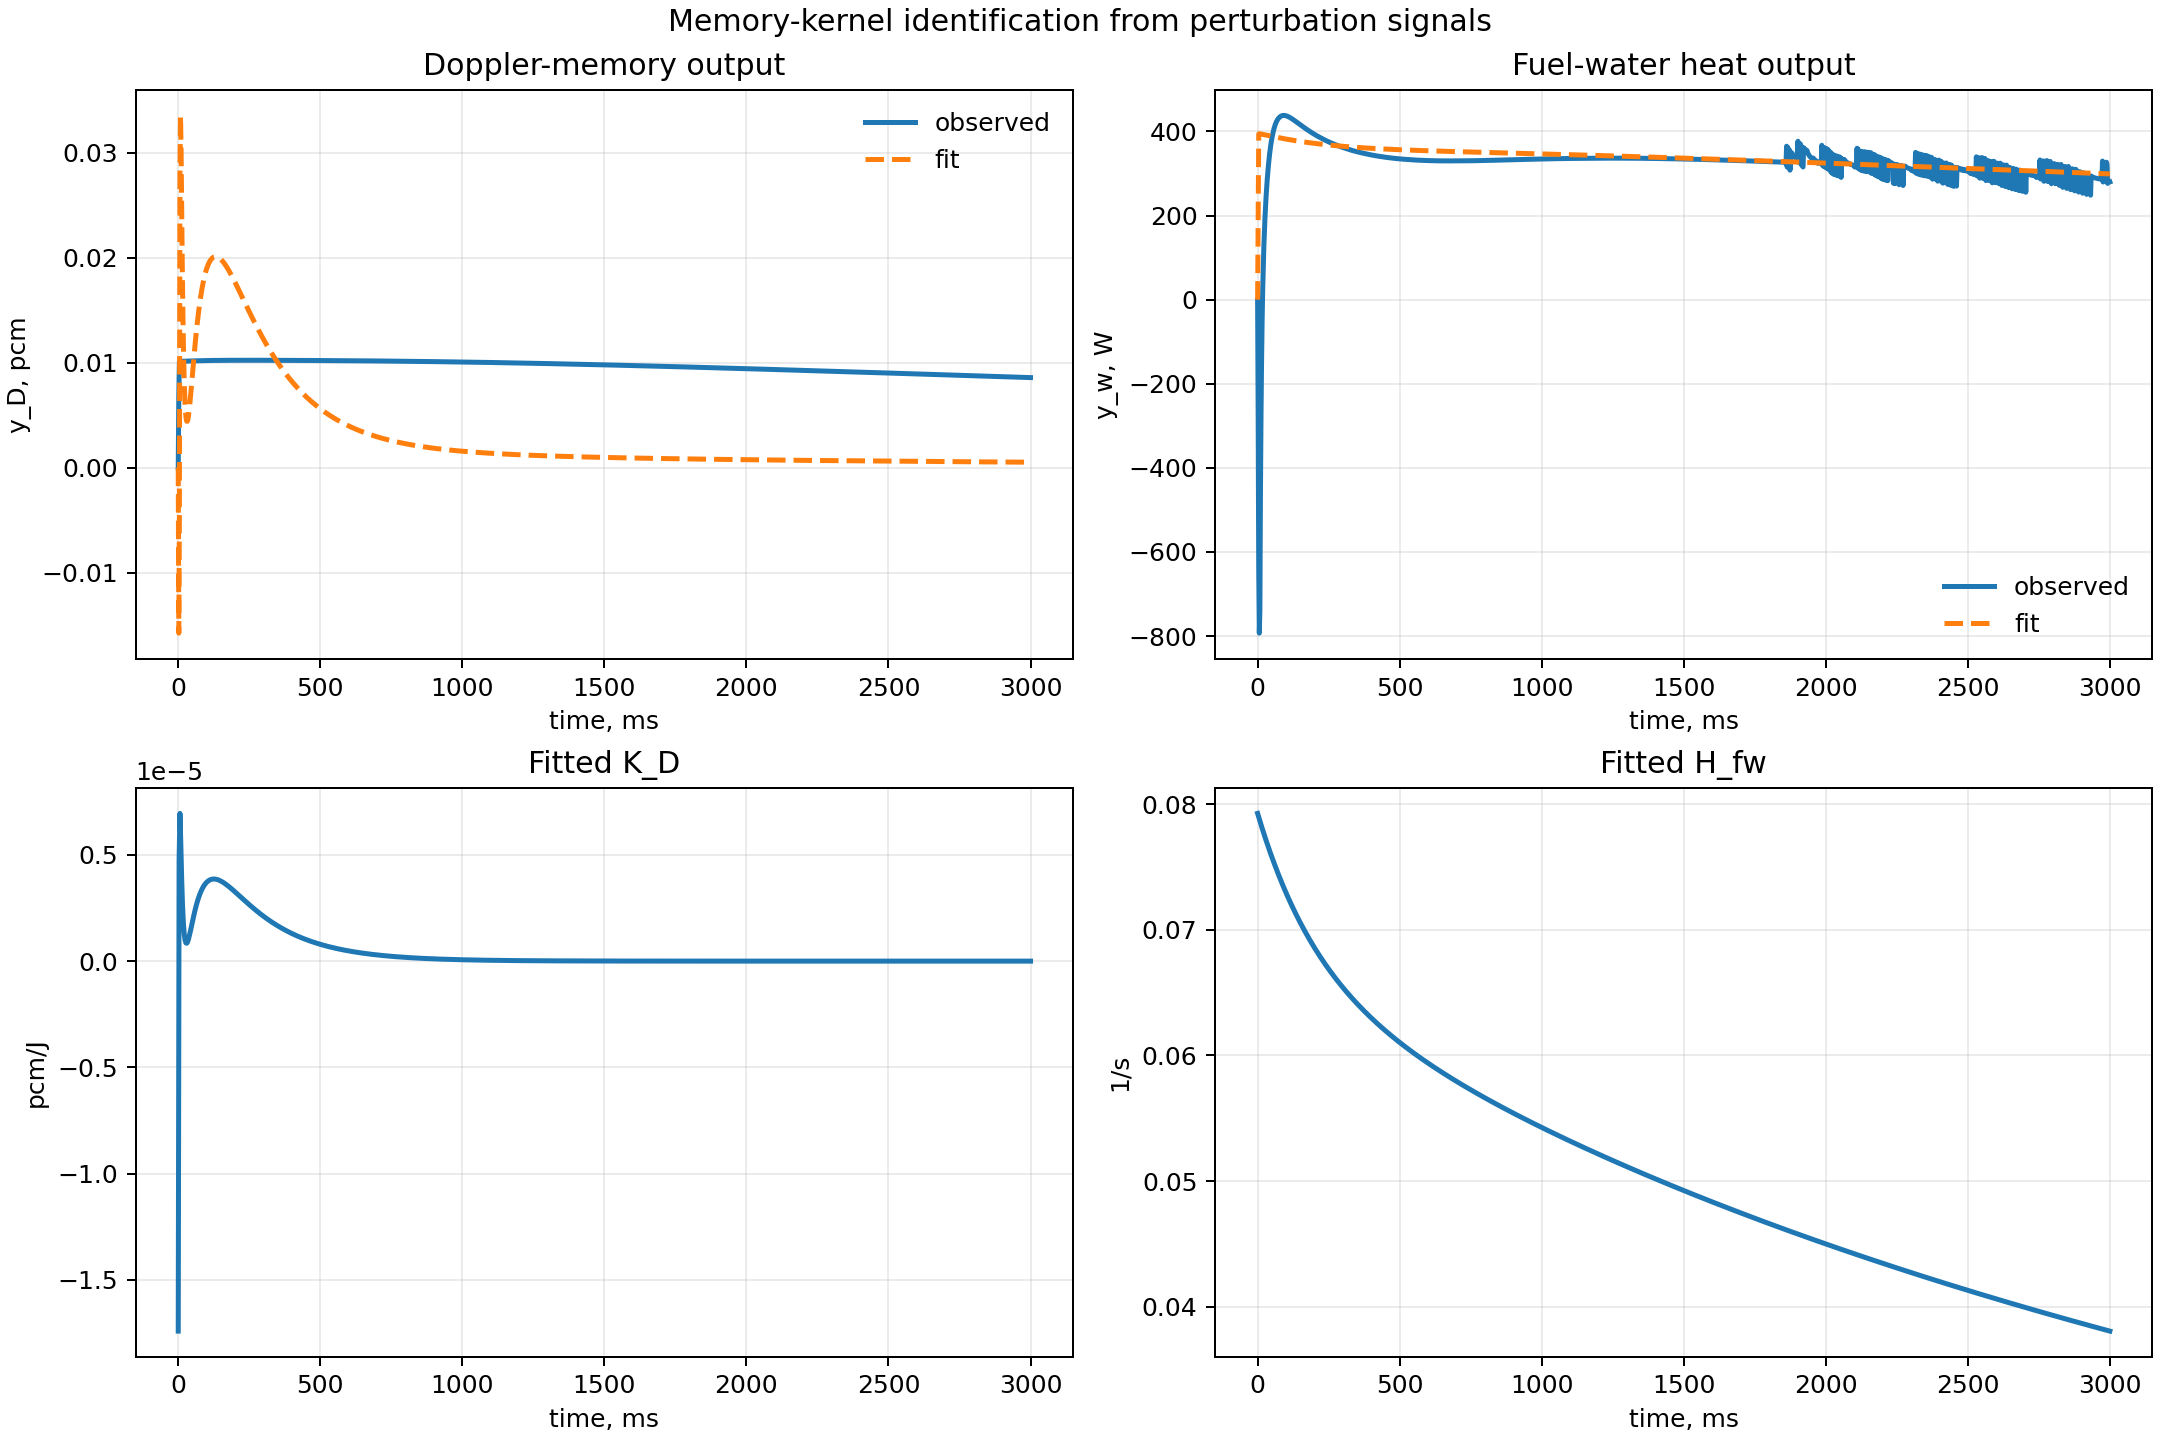
\includegraphics[width=\textwidth]{figures/fig10_kernel_fit.png}
    \caption{Joint fit экспоненциальных ядер: \(H_{fw}\) воспроизводится существенно лучше, чем \(K_D\). Sign-changing fit \(K_D\) показан как диагностика неидентифицируемости, а не как физическое реактивностное ядро.}
    \label{fig:kernelFit}
\end{figure}

Для проверки переносимости используется leave-one-out схема: ядро \(H_{fw}\) подбирается по четырём длительностям импульса и предсказывает пятую. Такая проверка важнее визуального совпадения, потому что показывает, что тепловой канал не просто подогнан под один график, а переносится между cases.

\begin{figure}[H]
    \centering
    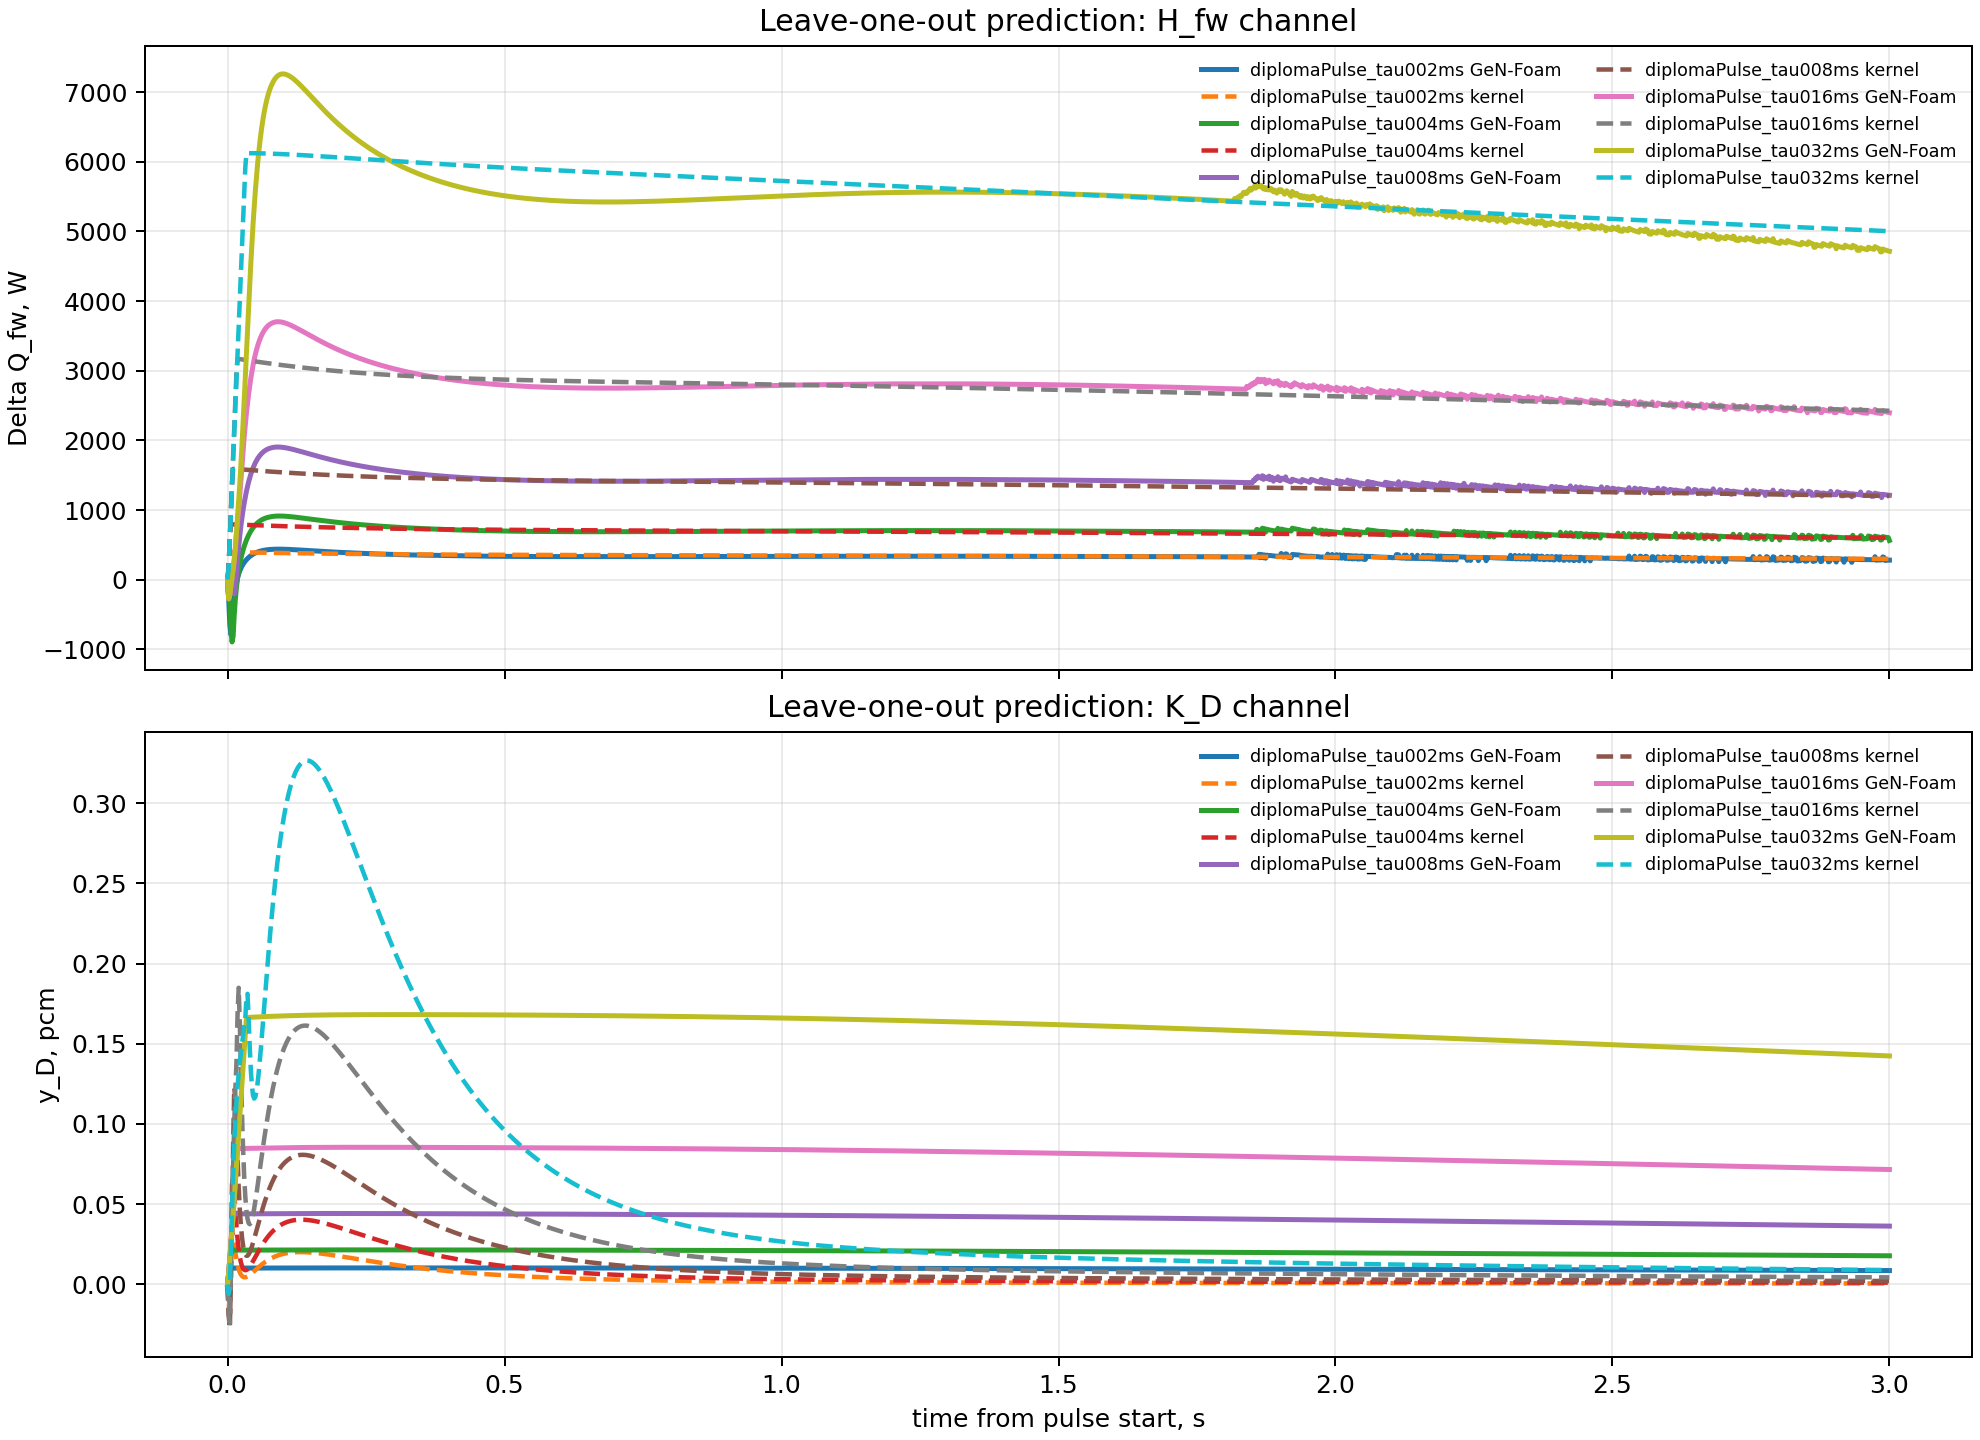
\includegraphics[width=\textwidth]{figures/fig11_leave_one_out_prediction.png}
    \caption{Leave-one-out prediction. Тепловой канал воспроизводит интегральные энергии лучше, чем ранний фронт; реактивностный канал остаётся слабо предсказуемым.}
    \label{fig:leaveOneOutPrediction}
\end{figure}

\section{Обсуждение}

Полученные результаты требуют аккуратной интерпретации. Теоретическая модель описывает режим, в котором твэл может работать как доплеровский элемент памяти: история мощности создаёт \(I_D=K_D*P\), а затем отрицательная реактивность ограничивает дальнейший рост мощности. Reduced-модель показывает такой целевой режим качественно. Однако GeN-Foam benchmark относится к другой области параметров: внешняя вставка реактивности доминирует, а топливная обратная связь мала.

Именно поэтому основной численный вывод состоит не в доказательстве самогашения, а в классификации режима. При
\[
\mathcal D_{\mathrm{ext}}=7.66\cdot10^{-4}
\]
текущий benchmark не может считаться доплеровски активным. Это ограничение не обесценивает расчёт: оно показывает, что предложенная диагностика различает целевой Doppler-active режим и слабосвязанный forced transient.

Положительный результат GeN-Foam части относится к тепловому каналу. Серия малых импульсов показывает, что \(H_{fw}\) может быть идентифицирован как линейное причинное ядро. При этом тепловая память оказывается секундной, а не миллисекундной. Поэтому в финальной версии работы важно не утверждать универсально \(\tau_H\sim10\)--\(100\,\mathrm{ms}\), а разделять идеализированную диффузионную оценку и effective \(H_{fw}\), полученный в конкретной sub-scale модели GeN-Foam.

Реактивностное ядро \(K_D\) в текущей постановке не идентифицируется надёжно. Корректная формулировка результата такова: \(H_{fw}\) восстановлено по диагностической серии, а для \(K_D\) получена только оценка слабой доплеровской активации. Для перехода к полноценной проверке \(K_D\) нужен отдельный Doppler-active benchmark, например controlled reduced model
\[
\rho_{\mathrm{eff}}(t)=
\rho_0-K_D*P,
\]
в котором \(\mathcal D_{\mathrm{ext}}\sim1\) и самогашение действительно формируется топливом.

Отдельно следует отметить численный noise floor по \(\rho_f\). В выполненной обработке есть только оценка гладкости самого \(y_D(t)\), но нет строгого шума из повторных no-pulse расчётов или независимого pre-pulse окна. Поэтому малость \(\max|\Delta\rho_f|=0.0442\,\mathrm{pcm}\) рассматривается как основание для классификации режима, но не как достаточная база для точного восстановления формы \(K_D(t)\).

Число \(\alpha_{\mathrm{eff}}=-0.300\,\mathrm{pcm/K}\), приведённое в таблице диагностики, также не следует трактовать как независимый статический коэффициент материала. В данной работе это transient-оценка по малому сигналу. Для самостоятельной верификации доплеровской физики требуются статические perturbation runs при \(T_f=T_0+\Delta T\) и независимое вычисление \(\Delta\rho/\Delta T\). В перспективе для этого подходит, например, OpenMC с windowed multipole representation для on-the-fly Doppler broadening \cite{OpenMCCrossSections}; в текущем тексте OpenMC рассматривается именно как возможный источник статических данных, а не как выполненная часть численного исследования.

Энергетическая интерпретация \(\mathcal W(3\,\mathrm{s})\approx0.135\)--\(0.140\) также ограничена уровнем доступных данных. Эта величина означает, что за \(3\,\mathrm{s}\) в sub-scale водный канал перешла указанная доля excess-энергии. Остальная энергия не считается потерянной: она остаётся в тепловой инерции топлива, оболочки, теплоносителя и численном остатке баланса. Полное закрытие баланса требует отдельной таблицы \(E_{\mathrm{pulse}}=\Delta E_f+\Delta E_{\mathrm{clad}}+\Delta E_c+E_w+\varepsilon\), которая выходит за рамки выполненной обработки.

\section{Заключение}

В работе построена двухканальная модель памяти твэла. История мощности преобразуется в два причинных функционала:
\[
I_D(t)=\int_0^tK_D(t-s)P(s)\,ds,
\qquad
Q_{fw}(t)=\int_0^tH_{fw}(t-s)P(s)\,ds.
\]
Первый функционал описывает доплеровскую реактивностную память топлива, второй -- задержанный тепловой поток в воду.

Построено геометрическое выражение для \(K_D\), связывающее форму энерговыделения, тепловую функцию Грина и поле доплеровской важности. Аналогично сформулировано ядро \(H_{fw}\), определяемое граничным тепловым функционалом на поверхности теплообмена. Введены диагностические параметры \(\mathcal D_{\mathrm{ext}}\), \(\mathcal D_\beta\) и \(\mathcal W(t_{\mathrm{obs}})\), позволяющие различать доплеровски активный режим и weak-coupled forced transient.

GeN-Foam benchmark классифицирован как слабосвязанный внешне вынужденный переходный процесс:
\[
\rho_{\mathrm{ext}}^{\max}=57.67\,\mathrm{pcm},
\qquad
\max|\Delta\rho_f|=0.0442\,\mathrm{pcm},
\qquad
\mathcal D_{\mathrm{ext}}=7.66\cdot10^{-4}.
\]
Следовательно, этот расчёт не доказывает доплеровское самогашение, но служит проверкой диагностики.

По диагностической серии импульсов \(\tau_p=2,\ 4,\ 8,\ 16,\ 32\,\mathrm{ms}\) показано, что тепловой канал \(H_{fw}\) идентифицируется устойчиво: нормированные тепловые отклики имеют близкую форму, joint fit даёт \(R^2\approx0.987\), а leave-one-out prediction подтверждает переносимость ядра. При этом к \(3\,\mathrm{s}\) в водный канал уходит около \(13.5\)--\(14.0\%\) excess-энергии, что указывает на секундную память теплового канала в данной GeN-Foam постановке.

Не доказаны в текущем GeN-Foam case сильное доплеровское самогашение, надёжное восстановление \(K_D\) и участие воды в формировании пика мощности. Эти ограничения являются частью результата: предложенная модель не только описывает целевой режим памяти твэла, но и даёт диагностику, показывающую, когда конкретный расчёт этому режиму не соответствует.

\newpage
\section{Список литературы}
\begin{thebibliography}{15}
    \bibitem{DuderstadtHamilton1976}
    Duderstadt J. J., Hamilton L. J. \textit{Nuclear Reactor Analysis}. Wiley, 1976.

    \bibitem{NRCFeedback2012}
    U.S. Nuclear Regulatory Commission. \textit{Module 10: Power Reactor Feedback Effects. Rev. 01}. 2012. URL: \href{https://www.nrc.gov/docs/ML1214/ML12142A130.pdf}{nrc.gov/docs/ML1214/ML12142A130.pdf}.

    \bibitem{DOEGeneralTechnicalBase2013}
    U.S. Department of Energy. \textit{General Technical Base Qualification Standard Reference Guide}. 2012. URL: \href{https://www.energy.gov/sites/prod/files/2013/10/f4/QSR-GeneralTechnicalBase.pdf}{energy.gov/sites/prod/files/2013/10/f4/QSR-GeneralTechnicalBase.pdf}.

    \bibitem{OpenMCCrossSections}
    OpenMC Documentation. \textit{Cross Section Representations}. URL: \href{https://docs.openmc.org/en/stable/methods/cross_sections.html}{docs.openmc.org/en/stable/methods/cross\_sections.html}.

    \bibitem{MOOSEHeatTransfer}
    MOOSE Framework. \textit{Heat Transfer Module}. URL: \href{https://mooseframework.inl.gov/modules/heat_transfer/}{mooseframework.inl.gov/modules/heat\_transfer}.

    \bibitem{OpenFOAMSolvers}
    OpenFOAM Documentation. \textit{Standard Solvers}. URL: \href{https://www.openfoam.com/documentation/user-guide/a-reference/a.1-standard-solvers}{openfoam.com/documentation/user-guide/a-reference/a.1-standard-solvers}.

    \bibitem{GeNFoam2015}
    Fiorina C., Clifford I., Aufiero M., Mikityuk K. GeN-Foam: A Novel OpenFOAM Based Multi-Physics Solver for 2D/3D Transient Analysis of Nuclear Reactors // \textit{Nuclear Engineering and Design}. 2015. Vol. 294. P. 24--37. DOI: \href{https://doi.org/10.1016/j.nucengdes.2015.05.035}{10.1016/j.nucengdes.2015.05.035}.

    \bibitem{foamForNuclear2026}
    Nervi G., Guilbaud T., Fiorina C., Hursin M., Scolaro A. foamForNuclear: A Unified OpenFOAM Multi-Physics Platform for Nuclear Applications // \textit{Progress in Nuclear Energy}. 2026. Vol. 193. Article 106250. DOI: \href{https://doi.org/10.1016/j.pnucene.2026.106250}{10.1016/j.pnucene.2026.106250}.
\end{thebibliography}

\end{document}
